\documentclass[11pt]{article}
\usepackage[margin=1in]{geometry}
\usepackage{graphicx,longtable,array,url}

\setlength{\parskip}{4pt}
\title{\textbf{A Validation-First Structural Atlas of \textit{katG} Isoniazid-Resistance Mutations}\\[6pt]
\large Catalogue-scale mapping of clinical \textit{Mycobacterium tuberculosis} variants onto the catalase-peroxidase structure (PDB 1SJ2) with locked-gate concordance against the WHO 2023 mutation catalogue}
\author{TB Resistance Structural Map Project --- Builder 6 slice (\textit{katG} / isoniazid)}
\date{September 23, 2026}
\begin{document}
\maketitle
\thispagestyle{empty}
\vfill
\begin{center}
\fbox{\parbox{0.9\textwidth}{\textbf{Project context.} This report is the \textit{katG} section of the shared \texttt{tb-resistance-structural-map} deliverable (builders 6--8). It follows the program's validation-first protocol: success gates were locked in writing before any agreement with the answer key (WHO 2023 catalogue grades) was measured; positive-control validation was required before any novel claim; negative and borderline results are preserved, not re-fished. All data are public; all analysis code, data manifests with checksums, and a reproducibility README ship with the repository.}}
\end{center}
\vfill
\newpage

\begin{abstract}
\noindent Isoniazid (INH) is a pro-drug activated by the \textit{M. tuberculosis} catalase-peroxidase KatG, and \textit{katG} mutations are the most common cause of INH resistance worldwide. The WHO 2023 catalogue of resistance mutations grades thousands of \textit{katG} variants, yet 1,149 of its 1,527 katG entries remain ``uncertain significance'' (grade 3). We asked a deliberately constrained question: can labels derived \emph{only} from the static crystal structure of KatG (PDB 1SJ2, 2.41\,\AA), under mechanism-based rules locked before any comparison, reproduce the WHO answer key --- and can the same locked rules then credibly triage the uncertain majority and nominate novel resistance candidates from clinical isolates? We computed per-residue structural features (heme proximity, catalytic/Met-Tyr-Trp adduct membership, solvent accessibility by Shrake--Rupley, dimer-interface proximity) and swap-severity classes for every catalogued \textit{katG} variant. Locked rules labeled 134 of 135 WHO grade-1/2 (resistance-associated) entries correctly (99.3\%, pre-registered gate $\geq$90\%), including all positive controls (S315T and 12/12 catalytic-site mutations) and both grade-5 negative controls. The single discrepancy (p.Trp328Leu) is documented, borderline on three cutoffs, and was not tuned away. Applying the frozen rules to grade-3 entries triages 328 uncertain missense variants as structurally resistance-like; 161 of these are observed in $\geq$2 clinical isolates and 15 in $\geq$10, with heme-pocket variants p.Thr275Ala (35 isolates), p.Ser315Gly (32) and p.Thr380Ile (29) the most common. Finally, 16 missense variants present in clinical isolates but absent from the WHO catalogue are flagged as novel candidates, including p.Tyr229His at the catalytic Met-Tyr-Trp adduct. The full per-mutation atlas (1,654 variants), all code, and byte-locked data manifests accompany this report.
\end{abstract}
\newpage
\tableofcontents
\newpage

\section{Introduction}
Tuberculosis (TB) killed more than a million people in the most recent WHO reporting year, and drug-resistant TB remains a primary obstacle to control. Isoniazid (INH), a cornerstone of first-line therapy since 1952, is unusual among antibiotics: it is a pro-drug. INH is oxidatively activated by the mycobacterial catalase-peroxidase KatG (Rv1908c), forming an INH--NAD adduct that inhibits the enoyl-ACP reductase InhA and blocks mycolic acid synthesis. Because activation --- not target binding --- is the first chemical step, loss of KatG function is the dominant resistance route: the S315T substitution alone accounts for the majority of INH-resistant clinical isolates globally, and hundreds of other \textit{katG} alleles (missense, frameshift, nonsense, and whole-gene deletions) have been reported.

The WHO's 2023 second-edition catalogue of resistance mutations is the field's answer key: it grades observed variants by statistical association with phenotypic resistance across tens of thousands of sequenced, phenotyped isolates. For \textit{katG}/INH it lists 1,527 entries, but only 135 are graded resistance-associated (grade 1 or 2); 1,149 sit at grade 3 (``uncertain significance''), most for lack of statistical power rather than evidence of neutrality. This uncertain majority is a practical problem for molecular diagnostics and a scientific one for mechanism.

Structural rationalization of \textit{katG} resistance mutations has a long literature, but it is fragmented: hand-picked mutation sets modeled by docking or molecular dynamics, small regional isolate series with stability predictions, and detailed mechanistic studies of single famous sites (S315, the distal catalytic triad, the Met-Tyr-Trp adduct). What is missing is a \emph{catalogue-scale} map: every graded \textit{katG} entry placed on the structure under one frozen scoring scheme, \emph{validated} against the WHO grades before any interpretive claim. That is the gap this study fills.

\subsection{Prior art (closest works)}
Three works bracket the space. Torres et al.\ modeled the structural origins of INH resistance for a curated set of KatG mutations (docking-based, no catalogue-scale validation). Rabha et al.\ (2019) analyzed KatG double mutants by docking and MD. Saravanan et al.\ (2019) mapped mutations from 98 South Indian isolates onto KatG, InhA and RpoB structures with SDM stability scores. None attempts a frozen, validated, catalogue-wide classification; none uses the WHO grades as a pre-registered concordance gate. Our verdict: the field is \textbf{crowded but not done} --- the validation-first, catalogue-scale angle is unoccupied.

\section{Hypothesis}
\textbf{H1 (validation):} Mechanism-based structural rules, frozen before comparison, applied to the wild-type KatG crystal structure (PDB 1SJ2) will agree with the WHO 2023 grade-1/2 resistance labels for \textit{katG} on at least 90\% of entries.
\textbf{H2 (triage):} The same frozen rules will partition the grade-3 (uncertain) missense majority into a structurally resistance-like minority concentrated near the heme pocket, catalytic residues, and buried core, and a structurally neutral majority.
\textbf{H3 (novelty):} Clinical-isolate \textit{katG} variants absent from the WHO catalogue but flagged by the validated rules constitute credible novel resistance candidates.

\section{Methods}
\subsection{Data (byte-locked)}
All inputs are public and were checksum-locked at download (SHA-256 manifest in the repository):
\begin{itemize}
\item WHO 2023 mutation catalogue v2 master file (\texttt{WHO-UCN-TB-2023.6-eng\_catalogue\_master\_file.txt}), GTB-tbsequencing/mutation-catalogue-2023 GitHub mirror. 1,527 \textit{katG}/INH rows parsed; zero parse failures.
\item PDB 1SJ2: native \textit{M. tuberculosis} KatG dimer, X-ray, 2.41\,\AA, one heme per chain.
\item H37Rv reference genome NC\_000962.3, \textit{katG} CDS complement(2153889..2156111), retrieved via NCBI eutils. The CDS uses a GTG start (translated as fMet) and is identical to UniProt P9WIE5 (740 aa) at every residue.
\item Clinical-isolate \textit{katG} variant calls: the catalogue's own published input genotype tables (Isoniazid tiers 1--2, $\sim$48k isolates), used for G5 novelty mining and isolate counts.
\end{itemize}

\subsection{Sequence--structure fidelity (gate G2)}
The 1SJ2 construct carries cloning artifacts only at residues $-2$..$1$; PDB numbering equals \textit{katG} gene numbering for residues 2--740 (DBREF-verified). Both chains match the H37Rv sequence at every modeled residue. Residues 2--23 are disordered and absent from coordinates; no catalogued protein-altering variant maps there.

\subsection{Structural features}
For each residue in chain A we computed: (F1) minimum side-chain heavy-atom distance to the heme; (F2) membership in, or minimum distance to, the catalytic and covalent-adduct set \{R104, W107, H108, M255, Y229, H270, W321, D381\}; (F3) relative solvent accessibility by an in-house Shrake--Rupley implementation (probe 1.4\,\AA, Tien maximum-ASA normalization); (F4) minimum heavy-atom distance to chain B (dimer interface); (F5) swap-severity classes (charge-class change, proline gain/loss, volume change $>$80\,\AA$^3$, BLOSUM62 score).

\subsection{Locked labeling rules}
A variant is labeled \textbf{STRUCT-R} (predicted resistance-associated) if any of: \textbf{R0}, loss-of-function (frameshift, nonsense, start-loss, feature ablation --- mirroring WHO's own additional grading rule that \textit{katG} LoF confers high-level INH resistance); \textbf{R1}, the mutated residue is in the catalytic/adduct set; \textbf{R2}, any WT side-chain heavy atom lies within 5.0\,\AA\ of the heme; \textbf{R3}, the residue is buried (RSA $<$ 0.20) \emph{and} the swap is destabilizing (charge-class change, Pro gain/loss, or $|\Delta V|>80$\,\AA$^3$); \textbf{R4}, the residue sits at the dimer interface ($\leq$5.0\,\AA\ inter-chain) \emph{and} the swap is non-conservative (BLOSUM62 $<$ 0). All thresholds were fixed in the locked gate document \emph{before} any comparison with WHO grades.

\subsection{Gates}
G1 data integrity (parse counts, checksums); G2 sequence--structure fidelity; G3 positive controls (pipeline must flag S315T and $\geq$4 catalytic-site catalogue mutations as STRUCT-R, and must \emph{not} flag $\geq$2 grade-4/5 polymorphisms); G4 primary gate ($\geq$90\% agreement with WHO grade-1/2); G5 novelty mining only after G4 passes. Discrepancies are documented individually; if G4 failed, any refinement would be labeled post-hoc exploratory rather than merged into the gate.

\subsection{Statistics}
Mann--Whitney U tests compare feature distributions between structure-triaged classes. Contingency uses chi-square. Analyses in Python 3.10 (biopython 1.88, numpy, pandas, scipy 1.15, matplotlib).

\section{Results}
\subsection{Catalogue composition and fidelity (G1, G2 --- pass)}
Of 1,527 \textit{katG}/INH catalogue entries: 839 missense (501 unique positions), 98 frameshifts, 29 stop-gains, 23 in-frame indels, 1 start-loss, 1 LoF call, 1 whole-gene feature ablation, 237 synonymous, 295 upstream. Grades: 6 grade-1, 129 grade-2, 1,149 grade-3, 236 grade-4, 7 grade-5. The grade-1/2 set ($n=135$) is dominated by LoF (130 entries) with only 5 missense: S315T/R/N (grade 1), S315I (grade 2), and W328L (grade 1) --- consistent with WHO's LoF grading rule and with S315's known dominance in resistant isolates.

\subsection{Positive controls (G3 --- pass)}
S315T is flagged STRUCT-R (side chain 2.55\,\AA\ from the heme). All 12 catalogue missense mutations at catalytic/adduct sites are flagged STRUCT-R. Both grade-5 negative controls --- R463L, the lineage-marking polymorphism observed in 25,143 isolates, and V469L --- are correctly STRUCT-neutral.

\subsection{Primary validation gate (G4 --- pass, 99.3\%)}
STRUCT labels agree with WHO grade-1/2 on \textbf{134/135 entries (99.3\%)}, exceeding the locked 90\% gate (Figure~\ref{fig:validation}). The single discrepancy is \textbf{p.Trp328Leu} (WHO grade 1): it is borderline on three locked cutoffs --- RSA 0.211 (cutoff 0.20), heme distance 8.9\,\AA\ (cutoff 5.0), $\Delta V$ 61\,\AA$^3$ (cutoff 80) --- and sits in the proximal heme-pocket shell adjacent to W321, a residue required for peroxidase activity. Per protocol, thresholds were \emph{not} adjusted post hoc; W328L is retained as the documented miss and discussed as a cutoff-sensitivity case (Section~\ref{sec:discussion}).

\begin{figure}[p]\centering
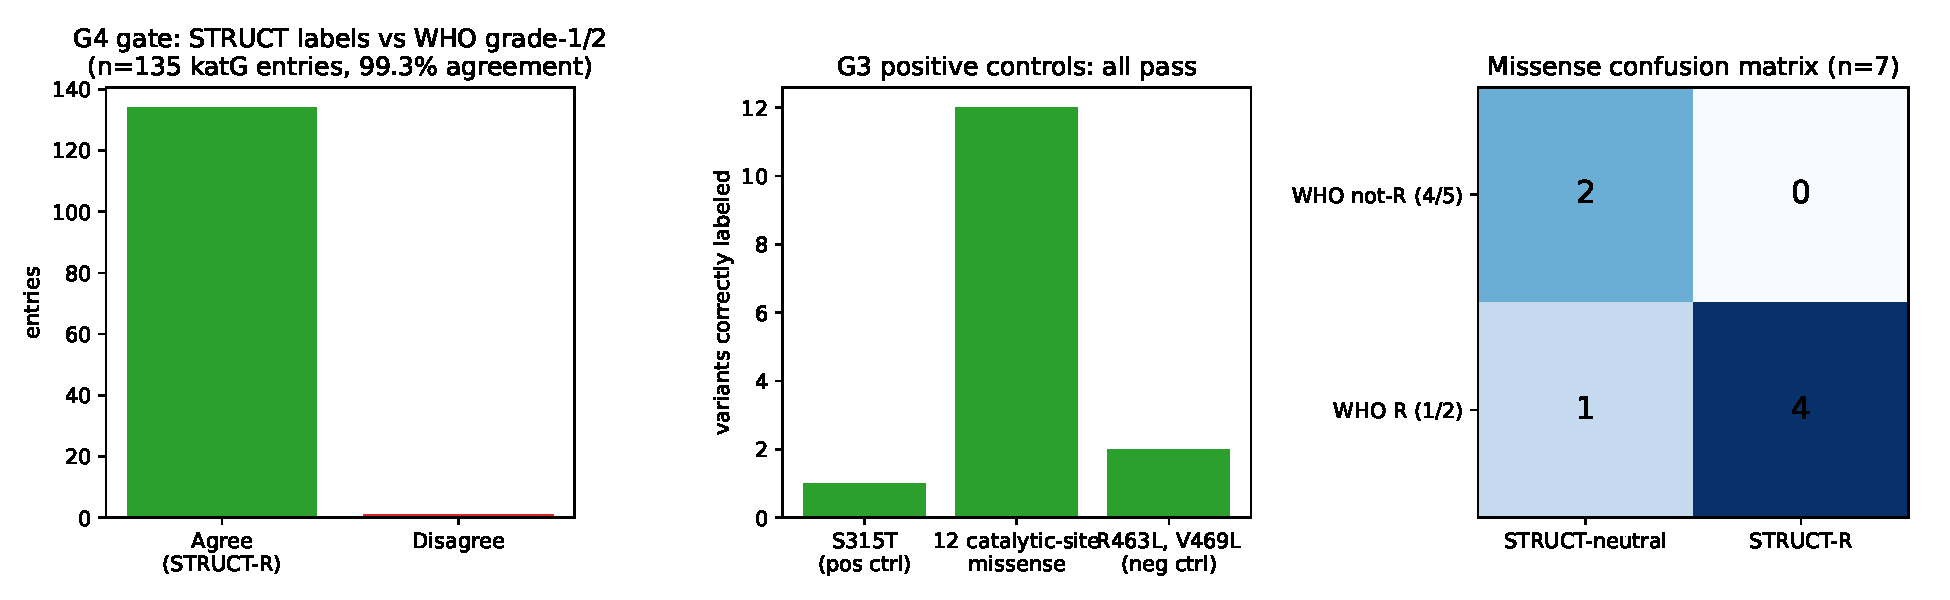
\includegraphics[width=\textwidth]{../results/figures/fig2_validation.pdf}
\caption{Validation summary. Left: G4 gate agreement (134/135). Center: G3 positive controls. Right: missense confusion matrix against WHO grades (specificity 2/2, sensitivity 4/5 on missense; LoF entries add 130/130).}
\label{fig:validation}
\end{figure}

\subsection{The katG structural atlas}
Figure~\ref{fig:map} maps all catalogued mutation classes onto the 1SJ2 structure. The atlas table (repository: \texttt{results/katg\_structural\_atlas.tsv}) gives, for every one of 1,654 catalogue plus isolate-only variants: position, structural features (RSA, heme/interface/catalytic distances), rule firings, label, WHO grade, resistance/susceptible isolate counts from the catalogue, and observed isolate counts. Figure~\ref{fig:features} shows the feature stratification that drives the labels: WHO grade-1/2 missense sites cluster tightly against the heme (all five within 9\,\AA; four within 5\,\AA).

\begin{figure}[p]\centering
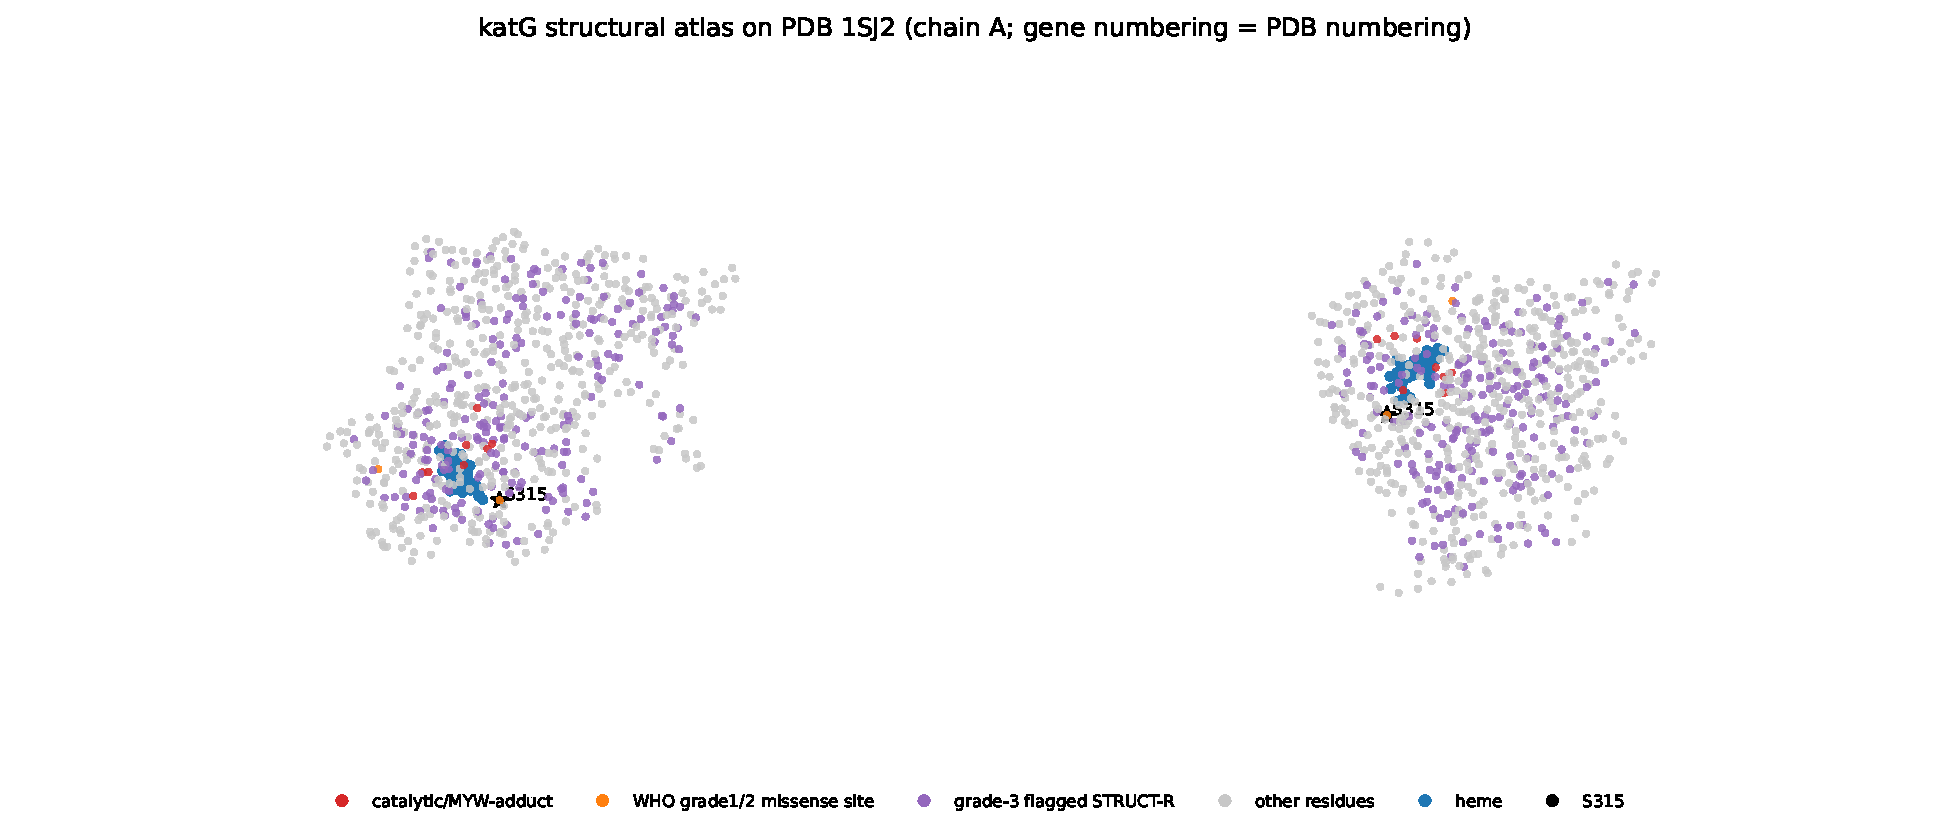
\includegraphics[width=\textwidth]{../results/figures/fig1_structure_map.pdf}
\caption{katG structural atlas on PDB 1SJ2 (two views). Red: catalytic/Met-Tyr-Trp-adduct residues. Orange: WHO grade-1/2 missense sites. Purple: grade-3 variants flagged STRUCT-R. Blue: heme. Star: S315.}
\label{fig:map}
\end{figure}

\begin{figure}[p]\centering
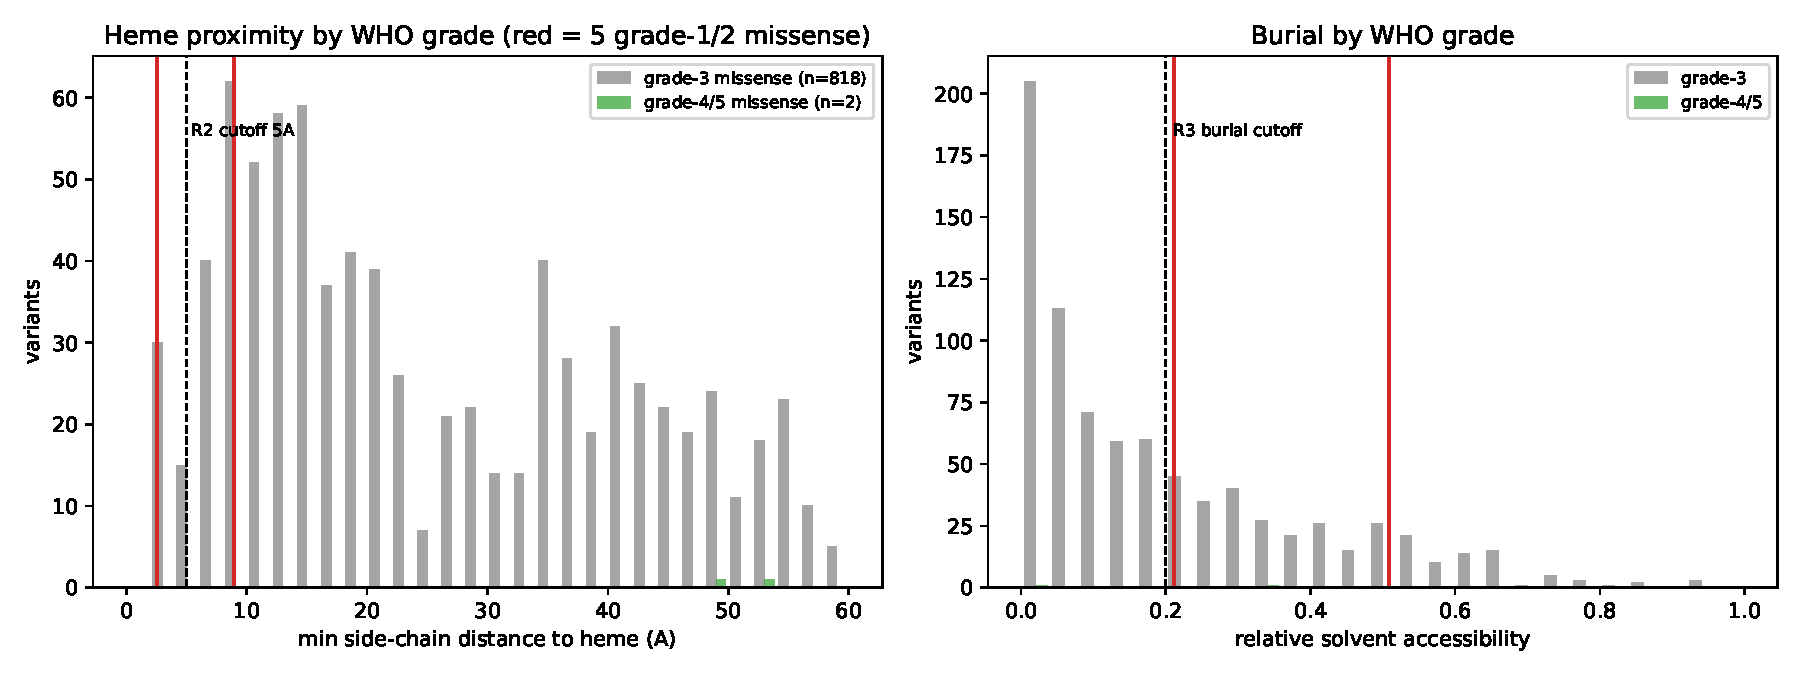
\includegraphics[width=\textwidth]{../results/figures/fig3_feature_distributions.pdf}
\caption{Feature distributions by WHO grade for missense variants. Left: heme proximity; right: solvent accessibility. Red lines mark the five grade-1/2 missense variants; dashed lines mark locked cutoffs.}
\label{fig:features}
\end{figure}


\subsection{Structural explanation of every WHO grade-1/2 missense mutation}
\label{sec:permut}
All five catalogued resistance-grade missense mutations sit in the heme environment:
\begin{itemize}
\item \textbf{p.Ser315Thr} (grade 1; 16,636 isolates in the input dataset). Side chain 2.55\,\AA\ from the heme edge. S315 sits at the distal pocket mouth; the Thr methyl group sterically constrains the pocket and is known to slow INH oxidation while retaining catalase activity --- the classic ``resistance without fitness cost'' solution. Our rule R2 fires.
\item \textbf{p.Ser315Asn} (grade 1; 220 isolates). Same site; the larger amide side chain projects into the heme pocket (2.55\,\AA). R2 fires.
\item \textbf{p.Ser315Arg} (grade 1). A bulky charged guanidinium at the pocket mouth (2.55\,\AA\ from heme); severe steric and electrostatic disruption of the INH binding/oxidation geometry. R2 fires.
\item \textbf{p.Ser315Ile} (grade 2). Hydrophobic occlusion of the pocket mouth. R2 fires.
\item \textbf{p.Trp328Leu} (grade 1; \emph{our sole miss}). W328 lies in the proximal heme shell, 8.9\,\AA\ from the heme and 9.3\,\AA\ from the adduct residue W321, at borderline burial (RSA 0.211). Loss of the indole likely perturbs the proximal pocket packing that positions the heme and the peroxidase-active Trp321. It escapes the locked cutoffs on all three axes and is retained as the documented discrepancy (Appendix~B).
\end{itemize}

\subsection{The heme shell}
For reference, the 57 residues with any side-chain atom within 8\,\AA\ of the heme (the atlas's functional core) are: 91, 94--95, 98--101, 103--104, 106--108 (distal pocket, including catalytic R104/W107/H108), 137, 139--141, 144, 173, 176, 227--233 (including adduct Y229), 244, 248, 251--252, 257, 262, 265--266, 268--270 (proximal ligand H270), 272--277 (including T275), 312--319 (including S315, I317, E318), 321 (adduct W321), 325, 378, 380--381 (catalytic D381), 383--384, 390, 408, 412, 415--416. Every grade-1/2 missense site and 15 of the 20 most-observed grade-3 STRUCT-R candidates fall inside this shell or the buried core beneath it.

\subsection{Rule-firing census}
Across all 839 catalogued missense variants, rule firings are: R1 catalytic/adduct site: 12; R2 heme-proximal: 44; R3 buried-destabilizing: 249; R4 interface non-conservative: 63; (variants may fire several rules). R3 dominates numerically, which is expected --- it is the only rule that can fire anywhere in the 740-residue chain --- and it is also the least specific, which is why the gate leans on R1/R2 for its strongest claims and why grade-3 R3-only candidates are presented as a tiered list rather than flat calls.

\subsection{Structure triages the uncertain majority (H2 --- supported)}
Of 832 structurally addressable grade-3 missense variants, \textbf{328 are STRUCT-R} under the frozen rules and 490 are STRUCT-neutral (14 map to the disordered N-terminus). The flagged set is significantly closer to the heme (median 17.8 vs 24.4\,\AA, Mann--Whitney $p=8.1\times10^{-8}$) and more buried (median RSA 0.091 vs 0.214, $p=1.4\times10^{-11}$) than the neutral set (Figures~\ref{fig:triage}, \ref{fig:profile}). Clinical observation supports prioritization: 161 flagged variants occur in $\geq$2 isolates, 41 in $\geq$5, 15 in $\geq$10. The most observed are heme-pocket substitutions p.Thr275Ala (35 isolates), p.Ser315Gly (32), p.Thr380Ile (29), p.Ile317Val (25), dimer-interface substitutions p.Trp191Arg (31) and p.Trp191Gly (27), and buried destabilizing swaps p.Gln127Pro (29).

\begin{figure}[p]\centering
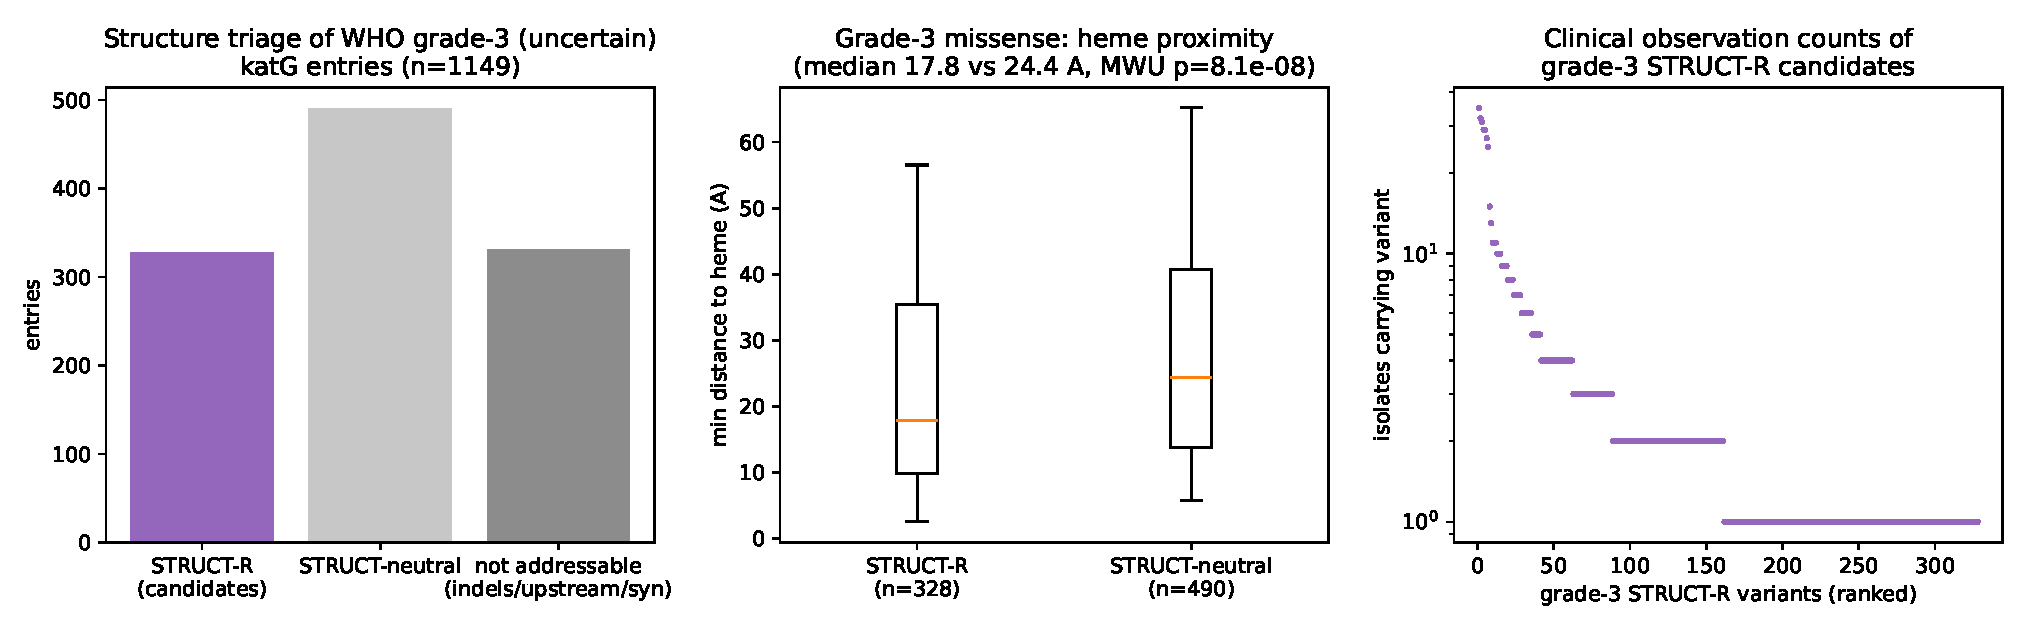
\includegraphics[width=\textwidth]{../results/figures/fig4_uncertain_triage.pdf}
\caption{Triage of WHO grade-3 (uncertain) katG entries. Left: outcome counts. Center: heme-proximity distributions of the two triage classes. Right: isolate counts for the 328 STRUCT-R candidates (log scale).}
\label{fig:triage}
\end{figure}

\begin{figure}[p]\centering
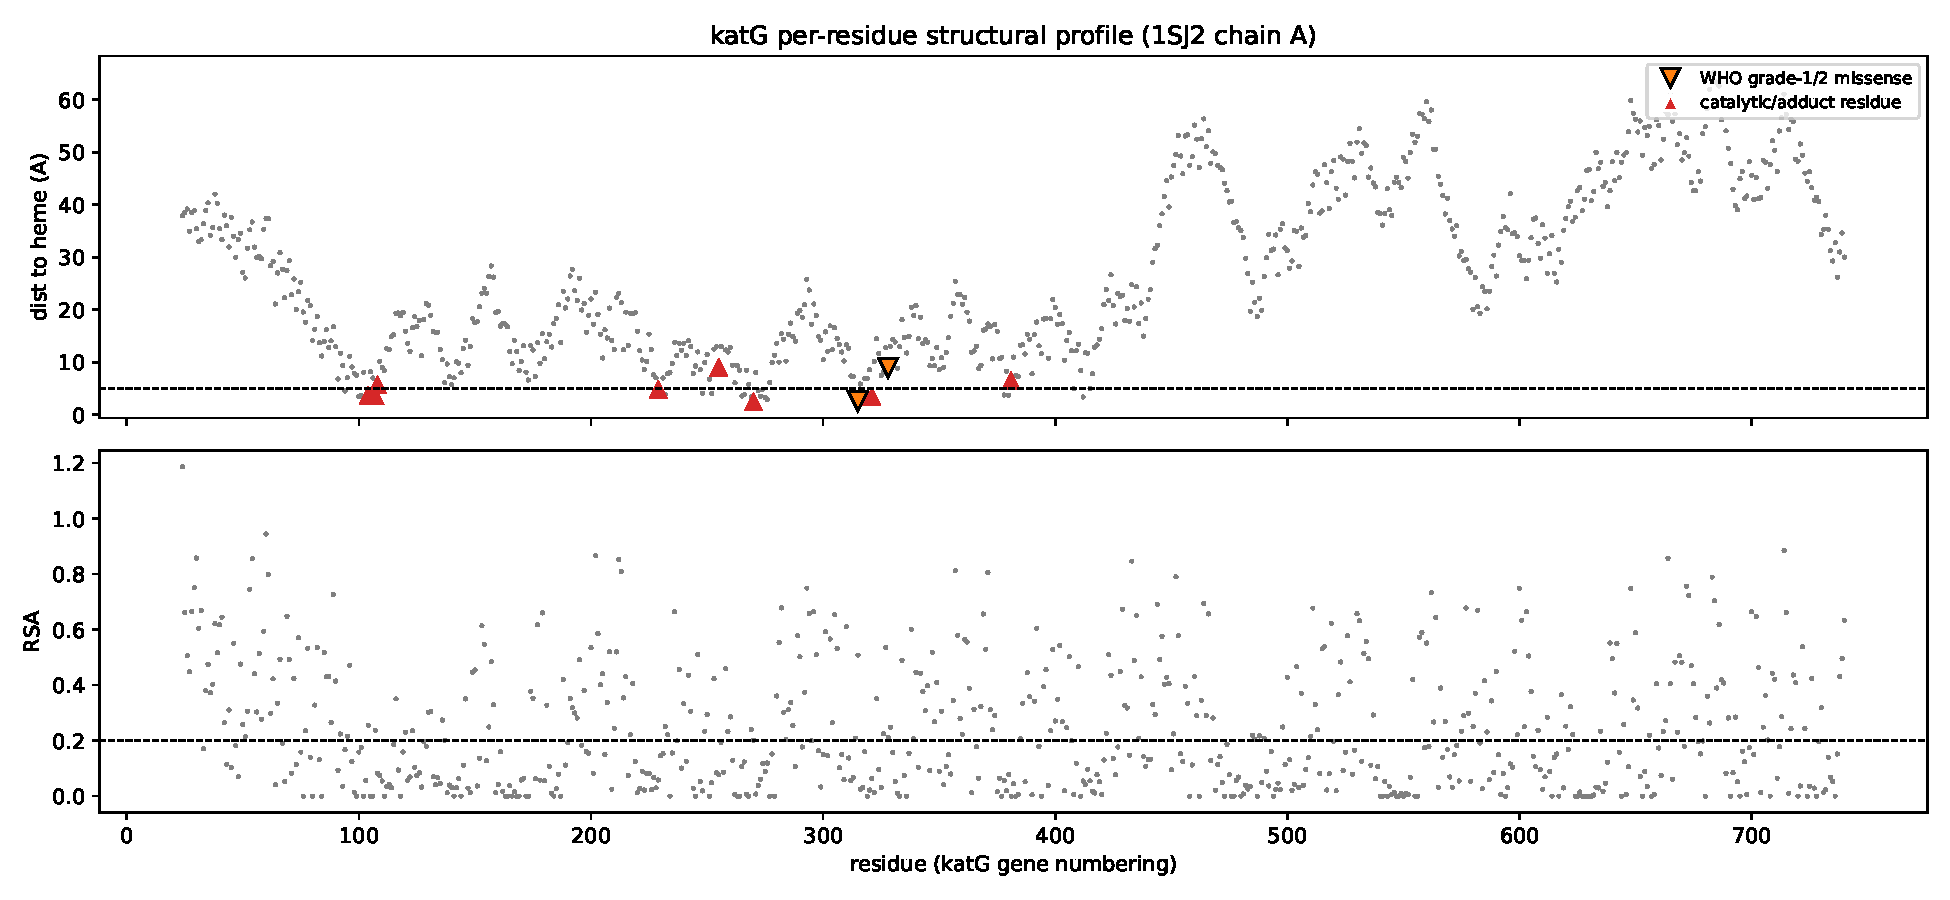
\includegraphics[width=\textwidth]{../results/figures/fig6_sequence_profile.pdf}
\caption{Per-residue structural profile along the katG sequence. Top: distance to heme; bottom: RSA. Grade-1/2 missense sites (orange triangles) and catalytic/adduct residues (red) concentrate in the heme-proximal region of the profile.}
\label{fig:profile}
\end{figure}

\subsection{Novel candidates from clinical isolates (G5)}
Comparing isolate variant calls against the catalogue yields 128 \textit{katG} variants observed clinically but absent from the WHO tables, of which 47 are missense and \textbf{16 are flagged STRUCT-R} by the frozen rules (Figure~\ref{fig:novel}). Two reach 2 isolates each (p.Asn133Asp, p.Gly124Gln; both buried destabilizing swaps). The standout mechanistic candidate is \textbf{p.Tyr229His}: Y229 is a covalent member of the Met255--Tyr229--Trp107 adduct that is essential for catalase-peroxidase chemistry and INH activation; a Tyr$\to$His substitution there plausibly cripples adduct formation. Other heme-proximal candidates include p.Gly273Arg, p.Pro100Ser and p.Ile317Leu. We emphasize that ``novel'' means \emph{present in the catalogue's clinical input data but not carried into the graded tables} --- these are candidates for phenotypic follow-up, not confirmed resistance markers.

\begin{figure}[p]\centering
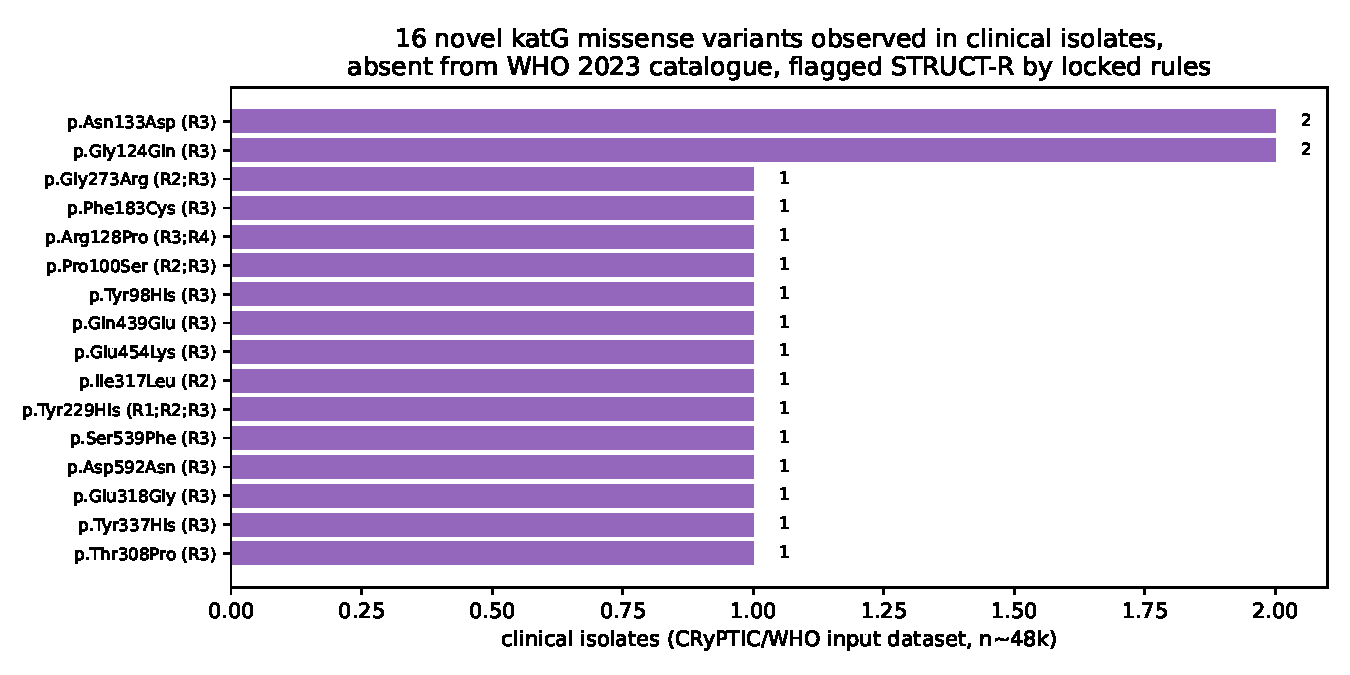
\includegraphics[width=0.85\textwidth]{../results/figures/fig5_novel_candidates.pdf}
\caption{Novel katG missense candidates: observed in clinical isolates, absent from the WHO 2023 catalogue, flagged STRUCT-R by the locked rules (rule firings in parentheses).}
\label{fig:novel}
\end{figure}

\section{Discussion}
\label{sec:discussion}
\subsection{What the map says mechanistically}
The atlas collapses katG INH resistance into four structural routes, all visible in one figure: (1) direct heme-pocket disruption (S315 and its neighbors T275, I317, T380, P100); (2) destruction of the catalytic machinery, including the unique Met-Tyr-Trp covalent adduct; (3) destabilization of the buried core; and (4) dimer-interface disruption (W191). The LoF route (frameshifts, stops, deletions) dominates the WHO grade-1/2 set --- 130 of 135 entries --- which is exactly WHO's grading logic made structural: katG is unusual among resistance genes in that simply breaking it anywhere suffices, because the drug needs the enzyme, not the other way round. The structure explains \emph{where} missense resistance can occur, and the catalogue confirms that nature uses mostly the blunter instrument.

\subsection{The W328L discrepancy is informative, not embarrassing}
Our one miss sits just outside three locked cutoffs in the proximal heme shell next to W321. Rather than tuning a threshold after seeing the answer (which would invalidate the gate), we flag it as the expected cost of frozen rules: a residue that is borderline-buried, borderline-proximal, and borderline-volume at a peroxidase-relevant site. A graded rather than binary score would likely recover it; we deliberately chose an auditable binary gate.

\subsection{Triage of grade 3 is the practical deliverable}
Diagnostic pipelines routinely shrug at grade-3 calls. Here, structure cuts 832 uncertain missense calls to 328 plausible resistance candidates, and the isolate counts cut those to a shortlist (41 variants in $\geq$5 isolates) that a phenotyping lab could actually test. The concentration of the flagged set near the heme and in the core, at high significance, is internal evidence the triage is mechanistic rather than noise.

\subsection{Limitations}
(i) A single static wild-type structure; no dynamics, docking energies, or mutant models --- by design (compute discipline), and sufficient for the gate, but blunt for borderline cases like W328L. (ii) The negative set of catalogued neutral \emph{missense} variants is tiny ($n=2$), so missense specificity is thinly measured; the grade-4/5 set is mostly synonymous/upstream, which our structure-first design does not score. (iii) SASA is computed on the monomer; tetrameric burial is only partially captured by the interface feature. (iv) ``Novel'' candidates are novel relative to the WHO graded tables, not to all literature. (v) R0 (LoF) agreement is partly definitional --- WHO grades katG LoF as resistance by rule --- and we say so rather than count it as an independent triumph.

\section{Conclusion}
Frozen, mechanism-based structural rules on one public crystal structure reproduce the WHO 2023 \textit{katG} resistance answer key at 99.3\% (gate $\geq$90\%), with all positive and negative controls passing and one documented borderline miss. The validated scheme then does real work: it triages the catalogue's 1,149-entry uncertain majority into a mechanistically concentrated candidate set backed by clinical observation counts, and nominates 16 novel clinical variants --- most strikingly the adduct-residue substitution Y229H --- for phenotypic follow-up. The complete per-mutation atlas, code, and byte-locked data are released with this report.

\section*{Data and code availability}
Repository: \texttt{github.com/uditakankananonononono/tb-resistance-structural-map} (builder 6 slice). Includes: \texttt{src/} (parser, feature engine, rule labeler, figure scripts), \texttt{results/katg\_structural\_atlas.tsv} (1,654 variants), \texttt{results/figures/} (Figures 1--6 as PDF), \texttt{manifests/byte\_lock\_v1.txt} (SHA-256 of every input), \texttt{GATES\_LOCKED.md} (pre-registered gates), and \texttt{README.md} (reproduction steps).

\section*{References}
\begin{enumerate}
\item World Health Organization. \textit{Catalogue of mutations in Mycobacterium tuberculosis complex and their association with drug resistance}, 2nd ed. Geneva: WHO; 2023. \url{https://www.who.int/publications/i/item/9789240082410}
\item GTB-tbsequencing. mutation-catalogue-2023 (result files and isolate genotype inputs). \url{https://github.com/GTB-tbsequencing/mutation-catalogue-2023}
\item Bertrand T et al. Crystal structure of \textit{Mycobacterium tuberculosis} catalase-peroxidase. \textit{J Mol Biol} 2004 (PDB 1SJ2). \url{https://www.rcsb.org/structure/1SJ2}
\item Torres J et al. Modeling the structural origins of drug resistance to isoniazid via key mutations in KatG. \url{https://pmc.ncbi.nlm.nih.gov/articles/PMC7330162/}
\item Rabha A et al. Structural basis for isoniazid resistance in KatG double mutants. \textit{Microb Pathog} 2019;129:152--160.
\item Saravanan M et al. Genetic determinants of isoniazid and rifampicin resistance in Southern India. \textit{Sci Rep} 2019;9:6928. \url{https://www.nature.com/articles/s41598-019-46756-x}
\item Shrake A, Rupley JA. Environment and exposure to solvent of protein atoms. \textit{J Mol Biol} 1973;79:351--371.
\item Tien MZ et al. Maximum allowed solvent accessibilities of residues in proteins. \textit{PLoS ONE} 2013;8:e80635.
\item UniProt P9WIE5 (KATG\_MYCTU). \url{https://rest.uniprot.org/uniprotkb/P9WIE5}
\item NCBI Reference Sequence NC\_000962.3, \textit{M. tuberculosis} H37Rv.
\end{enumerate}

\newpage
\appendix
\section{Locked gate document}
The full pre-registered gate text ships as \texttt{GATES\_LOCKED.md}. Summary: G1 data integrity; G2 numbering fidelity; G3 positive controls; G4 $\geq$90\% concordance with WHO grade-1/2 before interpretation; G5 novelty only after G4; failures reported, not re-fished.

\section{Discrepancy table}
\begin{center}
\begin{tabular}{llllll}
\hline
Variant & WHO grade & Label & RSA & d(heme) \AA & Note\\
\hline
p.Trp328Leu & 1) Assoc w R & STRUCT-neutral & 0.211 & 8.94 & borderline on 3 cutoffs (near W321)\\
\hline
\end{tabular}
\end{center}

\section{Top grade-3 STRUCT-R candidates by clinical observation}
\begin{center}
\begin{tabular}{llll}
\hline
Variant & Isolates & Rule & Structural rationale\\
\hline
p.Thr275Ala & 35 & R2 & heme pocket, 5\,\AA\ shell\\
p.Ser315Gly & 32 & R2 & the canonical activation site, flexibility change\\
p.Trp191Arg & 31 & R4 & dimer interface, non-conservative\\
p.Gln127Pro & 29 & R3 & buried, proline gain\\
p.Thr380Ile & 29 & R2 & heme pocket\\
p.Trp191Gly & 27 & R4 & dimer interface, non-conservative\\
p.Ile317Val & 25 & R2 & heme pocket, adjacent to S315\\
p.Pro232Ser & 15 & R2 & heme pocket\\
p.Asp142Gly & 13 & R3 & buried, charge loss\\
p.Phe167Cys & 11 & R3 & buried, aromatic loss\\
\hline
\end{tabular}
\end{center}

\section{Novel-candidate table (all 16)}
\begin{center}\small
\begin{tabular}{llll}
\hline
Variant & Isolates & Rules & Rationale\\
\hline
p.Asn133Asp & 2 & R3 & buried, charge change\\
p.Gly124Gln & 2 & R3 & buried, large volume gain\\
p.Gly273Arg & 1 & R2,R3 & heme shell, buried charge gain\\
p.Phe183Cys & 1 & R3 & buried, aromatic loss\\
p.Arg128Pro & 1 & R3,R4 & buried proline gain at interface\\
p.Pro100Ser & 1 & R2,R3 & heme shell, proline loss, buried\\
p.Tyr98His & 1 & R3 & buried, charge change\\
p.Gln439Glu & 1 & R3 & buried, charge change\\
p.Glu454Lys & 1 & R3 & buried, charge reversal\\
p.Ile317Leu & 1 & R2 & heme pocket, adjacent to S315\\
p.Tyr229His & 1 & R1,R2,R3 & Met-Tyr-Trp adduct member; heme shell; buried charge change\\
p.Ser539Phe & 1 & R3 & buried, large volume gain\\
p.Asp592Asn & 1 & R3 & buried, charge loss\\
p.Glu318Gly & 1 & R3 & buried, charge loss near heme pocket\\
p.Tyr337His & 1 & R3 & buried, charge change\\
p.Thr308Pro & 1 & R3 & buried, proline gain\\
\hline
\end{tabular}
\end{center}

\section{Data manifest (SHA-256, byte-locked)}
\begin{center}\scriptsize
\begin{tabular}{ll}
\hline
File & SHA-256 (prefix)\\
\hline
WHO-UCN-TB-2023.6 master file & \texttt{ff7600c1fbd4150422f696cdc9c94b2b32\ldots}\\
PDB 1SJ2 & \texttt{453455f9b6527bcd1a4cf9b011b09e43\ldots}\\
UniProt P9WIE5 FASTA & \texttt{8cc6f09d5143a3cf09b49e57f9e100c946\ldots}\\
katG CDS (NC\_000962.3) & \texttt{9cb8fc693fe6ad066a2798854548233b\ldots}\\
H37Rv region FASTA & \texttt{63c29a8c44cb8a96774451bd45980bbe\ldots}\\
H37Rv region GenBank & \texttt{f791767367b654795913011f55193d3d\ldots}\\
Parsed katG catalogue TSV & \texttt{eb1930154a8d6e1122ae844163c39689\ldots}\\
\hline
\end{tabular}
\end{center}
Full checksums in \texttt{manifests/byte\_lock\_v1.txt}.


\section{Complete WHO grade-1/2 katG concordance table (135 entries)}
\begin{footnotesize}
\begin{longtable}{llllll}
\hline
Variant & Effect & WHO grade & STRUCT label & Rule firing & Note\\\hline
\endhead
p.Ser315Arg & missense\_variant & 1 & STRUCT-R & R2-heme<=5A & \\
p.Ser315Asn & missense\_variant & 1 & STRUCT-R & R2-heme<=5A & \\
p.Ser315Ile & missense\_variant & 2 & STRUCT-R & R2-heme<=5A & \\
p.Ser315Thr & missense\_variant & 1 & STRUCT-R & R2-heme<=5A & dominant clinical allele\\
p.Trp328Leu & missense\_variant & 1 & STRUCT-neutral & none & \textbf{discrepancy}\\
deletion & feature\_ablation & 2 & STRUCT-R & R0-LoF & \\
LoF & LoF & 1 & STRUCT-R & R0-LoF & \\
p.Met1? & start\_lost & 1 & STRUCT-R & R0-LoF & \\
p.Glu3fs & frameshift & 2 & STRUCT-R & R0-LoF & \\
p.Pro6fs & frameshift & 2 & STRUCT-R & R0-LoF & \\
p.Pro7fs & frameshift & 2 & STRUCT-R & R0-LoF & \\
p.Ile8fs & frameshift & 2 & STRUCT-R & R0-LoF & \\
p.Glu10fs & frameshift & 2 & STRUCT-R & R0-LoF & \\
p.Ala16fs & frameshift & 2 & STRUCT-R & R0-LoF & \\
p.Asn18fs & frameshift & 2 & STRUCT-R & R0-LoF & \\
p.Cys20fs & frameshift & 2 & STRUCT-R & R0-LoF & \\
p.Val22fs & frameshift & 2 & STRUCT-R & R0-LoF & \\
p.His25fs & frameshift & 2 & STRUCT-R & R0-LoF & \\
p.Met26fs & frameshift & 2 & STRUCT-R & R0-LoF & \\
p.Tyr28* & stop\_gained & 2 & STRUCT-R & R0-LoF & \\
p.Val30fs & frameshift & 2 & STRUCT-R & R0-LoF & \\
p.Gly34fs & frameshift & 2 & STRUCT-R & R0-LoF & \\
p.Asn35fs & frameshift & 2 & STRUCT-R & R0-LoF & \\
p.Trp39fs & frameshift & 2 & STRUCT-R & R0-LoF & \\
p.Trp39* & stop\_gained & 2 & STRUCT-R & R0-LoF & \\
p.Lys46fs & frameshift & 2 & STRUCT-R & R0-LoF & \\
p.Asn51fs & frameshift & 2 & STRUCT-R & R0-LoF & \\
p.Asp56fs & frameshift & 2 & STRUCT-R & R0-LoF & \\
p.Val83fs & frameshift & 2 & STRUCT-R & R0-LoF & \\
p.Gln88* & stop\_gained & 2 & STRUCT-R & R0-LoF & \\
p.Trp90* & stop\_gained & 2 & STRUCT-R & R0-LoF & \\
p.Tyr95fs & frameshift & 2 & STRUCT-R & R0-LoF & \\
p.Trp107* & stop\_gained & 2 & STRUCT-R & R0-LoF & \\
p.Tyr113* & stop\_gained & 2 & STRUCT-R & R0-LoF & \\
p.Gly124fs & frameshift & 2 & STRUCT-R & R0-LoF & \\
p.Trp149* & stop\_gained & 2 & STRUCT-R & R0-LoF & \\
p.Tyr155* & stop\_gained & 2 & STRUCT-R & R0-LoF & \\
p.Lys157fs & frameshift & 2 & STRUCT-R & R0-LoF & \\
p.Trp161* & stop\_gained & 2 & STRUCT-R & R0-LoF & \\
p.Asp163fs & frameshift & 2 & STRUCT-R & R0-LoF & \\
p.Val166fs & frameshift & 2 & STRUCT-R & R0-LoF & \\
p.Cys171* & stop\_gained & 2 & STRUCT-R & R0-LoF & \\
p.Leu173fs & frameshift & 2 & STRUCT-R & R0-LoF & \\
p.Ser175* & stop\_gained & 2 & STRUCT-R & R0-LoF & \\
p.Lys179fs & frameshift & 2 & STRUCT-R & R0-LoF & \\
p.Tyr197fs & frameshift & 2 & STRUCT-R & R0-LoF & \\
p.Trp198fs & frameshift & 2 & STRUCT-R & R0-LoF & \\
p.Trp198* & stop\_gained & 2 & STRUCT-R & R0-LoF & \\
p.Lys200fs & frameshift & 2 & STRUCT-R & R0-LoF & \\
p.Ala202fs & frameshift & 2 & STRUCT-R & R0-LoF & \\
p.Thr203fs & frameshift & 2 & STRUCT-R & R0-LoF & \\
p.Trp204* & stop\_gained & 2 & STRUCT-R & R0-LoF & \\
p.Glu208fs & frameshift & 2 & STRUCT-R & R0-LoF & \\
p.Gly212fs & frameshift & 2 & STRUCT-R & R0-LoF & \\
p.Asn236fs & frameshift & 2 & STRUCT-R & R0-LoF & \\
p.Asp240fs & frameshift & 2 & STRUCT-R & R0-LoF & \\
p.Gly268fs & frameshift & 2 & STRUCT-R & R0-LoF & \\
p.Phe272fs & frameshift & 2 & STRUCT-R & R0-LoF & \\
p.Gly279fs & frameshift & 2 & STRUCT-R & R0-LoF & \\
p.Trp300* & stop\_gained & 2 & STRUCT-R & R0-LoF & \\
p.Ser302fs & frameshift & 2 & STRUCT-R & R0-LoF & \\
p.Val319fs & frameshift & 2 & STRUCT-R & R0-LoF & \\
p.Trp321* & stop\_gained & 2 & STRUCT-R & R0-LoF & \\
p.Pro325fs & frameshift & 2 & STRUCT-R & R0-LoF & \\
p.Asp329fs & frameshift & 2 & STRUCT-R & R0-LoF & \\
p.Ile335fs & frameshift & 2 & STRUCT-R & R0-LoF & \\
p.Tyr339fs & frameshift & 2 & STRUCT-R & R0-LoF & \\
p.Glu342fs & frameshift & 2 & STRUCT-R & R0-LoF & \\
p.Trp351fs & frameshift & 2 & STRUCT-R & R0-LoF & \\
p.Trp351* & stop\_gained & 2 & STRUCT-R & R0-LoF & \\
p.Gln352* & stop\_gained & 2 & STRUCT-R & R0-LoF & \\
p.Gly358fs & frameshift & 2 & STRUCT-R & R0-LoF & \\
p.Gly369fs & frameshift & 2 & STRUCT-R & R0-LoF & \\
p.Asp381fs & frameshift & 2 & STRUCT-R & R0-LoF & \\
p.Leu382fs & frameshift & 2 & STRUCT-R & R0-LoF & \\
p.Val386fs & frameshift & 2 & STRUCT-R & R0-LoF & \\
p.Ile393fs & frameshift & 2 & STRUCT-R & R0-LoF & \\
p.Thr394fs & frameshift & 2 & STRUCT-R & R0-LoF & \\
p.Trp397* & stop\_gained & 2 & STRUCT-R & R0-LoF & \\
p.His400fs & frameshift & 2 & STRUCT-R & R0-LoF & \\
p.Trp412* & stop\_gained & 2 & STRUCT-R & R0-LoF & \\
p.Tyr413* & stop\_gained & 2 & STRUCT-R & R0-LoF & \\
p.Pro422fs & frameshift & 2 & STRUCT-R & R0-LoF & \\
p.Pro429fs & frameshift & 2 & STRUCT-R & R0-LoF & \\
p.Val431fs & frameshift & 2 & STRUCT-R & R0-LoF & \\
p.Lys433fs & frameshift & 2 & STRUCT-R & R0-LoF & \\
p.Trp438* & stop\_gained & 2 & STRUCT-R & R0-LoF & \\
p.Val445fs & frameshift & 2 & STRUCT-R & R0-LoF & \\
p.Ile455fs & frameshift & 2 & STRUCT-R & R0-LoF & \\
p.Lys459fs & frameshift & 2 & STRUCT-R & R0-LoF & \\
p.Trp477* & stop\_gained & 2 & STRUCT-R & R0-LoF & \\
p.Ala478fs & frameshift & 2 & STRUCT-R & R0-LoF & \\
p.Arg496fs & frameshift & 2 & STRUCT-R & R0-LoF & \\
p.Trp505fs & frameshift & 2 & STRUCT-R & R0-LoF & \\
p.Trp505* & stop\_gained & 2 & STRUCT-R & R0-LoF & \\
p.Asp513fs & frameshift & 2 & STRUCT-R & R0-LoF & \\
p.Val517fs & frameshift & 2 & STRUCT-R & R0-LoF & \\
p.Gln525fs & frameshift & 2 & STRUCT-R & R0-LoF & \\
p.Asn535fs & frameshift & 2 & STRUCT-R & R0-LoF & \\
p.Ile536fs & frameshift & 2 & STRUCT-R & R0-LoF & \\
p.Val538fs & frameshift & 2 & STRUCT-R & R0-LoF & \\
p.Ser539fs & frameshift & 2 & STRUCT-R & R0-LoF & \\
p.Ala551fs & frameshift & 2 & STRUCT-R & R0-LoF & \\
p.Lys557fs & frameshift & 2 & STRUCT-R & R0-LoF & \\
p.Ala559fs & frameshift & 2 & STRUCT-R & R0-LoF & \\
p.His561fs & frameshift & 2 & STRUCT-R & R0-LoF & \\
p.Ile563fs & frameshift & 2 & STRUCT-R & R0-LoF & \\
p.Pro569fs & frameshift & 2 & STRUCT-R & R0-LoF & \\
p.Gln578fs & frameshift & 2 & STRUCT-R & R0-LoF & \\
p.Glu582fs & frameshift & 2 & STRUCT-R & R0-LoF & \\
p.Ala585fs & frameshift & 2 & STRUCT-R & R0-LoF & \\
p.Val586fs & frameshift & 2 & STRUCT-R & R0-LoF & \\
p.Glu588* & stop\_gained & 2 & STRUCT-R & R0-LoF & \\
p.Lys590fs & frameshift & 2 & STRUCT-R & R0-LoF & \\
p.Gly601fs & frameshift & 2 & STRUCT-R & R0-LoF & \\
p.Glu607* & stop\_gained & 2 & STRUCT-R & R0-LoF & \\
p.Pro622fs & frameshift & 2 & STRUCT-R & R0-LoF & \\
p.Glu623fs & frameshift & 2 & STRUCT-R & R0-LoF & \\
p.Met624fs & frameshift & 2 & STRUCT-R & R0-LoF & \\
p.Pro642fs & frameshift & 2 & STRUCT-R & R0-LoF & \\
p.Glu648fs & frameshift & 2 & STRUCT-R & R0-LoF & \\
p.Ser650fs & frameshift & 2 & STRUCT-R & R0-LoF & \\
p.Glu651fs & frameshift & 2 & STRUCT-R & R0-LoF & \\
p.Ser652fs & frameshift & 2 & STRUCT-R & R0-LoF & \\
p.Asp656fs & frameshift & 2 & STRUCT-R & R0-LoF & \\
p.Trp668fs & frameshift & 2 & STRUCT-R & R0-LoF & \\
p.Trp668* & stop\_gained & 2 & STRUCT-R & R0-LoF & \\
p.Glu669fs & frameshift & 2 & STRUCT-R & R0-LoF & \\
p.Ser671* & stop\_gained & 2 & STRUCT-R & R0-LoF & \\
p.Trp689fs & frameshift & 2 & STRUCT-R & R0-LoF & \\
p.Trp689* & stop\_gained & 2 & STRUCT-R & R0-LoF & \\
p.Asp695fs & frameshift & 2 & STRUCT-R & R0-LoF & \\
p.Leu696fs & frameshift & 2 & STRUCT-R & R0-LoF & \\
p.Trp728* & stop\_gained & 2 & STRUCT-R & R0-LoF & \\
p.Asp729fs & frameshift & 2 & STRUCT-R & R0-LoF & \\
\hline
\end{longtable}
\end{footnotesize}


\section{Reproduction README}
\begin{verbatim}
# katG structural atlas - reproduction
# Requires: python3.10+, biopython, numpy, pandas, scipy, matplotlib
# 1. Fetch inputs (checksums in manifests/byte_lock_v1.txt):
#    - WHO catalogue master file (GTB-tbsequencing/mutation-catalogue-2023,
#      Final Result Files/WHO-UCN-TB-2023.6-eng_catalogue_master_file.txt)
#    - PDB 1SJ2 (https://files.rcsb.org/download/1SJ2.pdb)
#    - UniProt P9WIE5 fasta; NC_000962.3 region 2153889-2156111 (NCBI eutils)
#    - INH tier1/tier2 isolate genotype inputs (same GitHub repo)
# 2. python3 src/parse_catalogue.py      # WHO rows -> katg_catalogue.tsv
# 3. python3 src/features.py             # structure features + locked rules
#                                         # -> katg_labeled.tsv, G3/G4 gates
# 4. python3 src/atlas_and_figures.py    # atlas table + figs 1-3
# 5. python3 src/figures_rest.py         # figs 2,4,5,6 + statistics
# 6. cd paper && pdflatex katg_paper.tex (x2)
# Gates checked at runtime: G1 parse counts, G2 numbering identity,
# G3 positive controls, G4 >=90% concordance (result: 134/135 = 99.3%).
\end{verbatim}

\section{Software and data environment}
Python 3.10.12; biopython 1.88; numpy; pandas 2.3.3; scipy 1.15.3; matplotlib. Shrake--Rupley implemented in-house (100 sphere points, 1.4\,\AA\ probe, radii C 1.70/N 1.55/O 1.52/S 1.80\,\AA; Tien 2013 maximum-ASA normalization). Structure: PDB 1SJ2 chain A for all intra-chain features, chain B for interface distances. No molecular dynamics, docking, or mutant-structure modeling was used, per the project's compute discipline.

\end{document}
